\chapter{State of the Art \& Related Work\label{cha:chapter2}}

This chapter presents the most relevant solutions existing in the field of blockchain scalability and explains the project this thesis is based on.
\section{Scalability solutions}
There are many ideas around the possible path to take to scale the blockchain. Some of them have already been implemented, while others are still in the research phase.

There are two main branches to scale the blockchain: Layer 1 and Layer 2 \cite{tyagi_study_2021,thibault_blockchain_2022}. Layer 1 solutions are those that scale the blockchain by increasing the block size or using Sharding. Layer 2 solutions are those that scale the blockchain by moving the computation off-chain. Some examples of Layer 2 solutions are State Channels, Sidechains and Rollups, as showed in Figure \ref{fig:2_scalingSolutions}.

The general followed path to scale the blockchain is to use a Layer 2 solution. This is the path that is being followed by most of the Ethereum community \cite{neiheiser_practical_2023}.

\begin{figure}[ht]
  \centering
  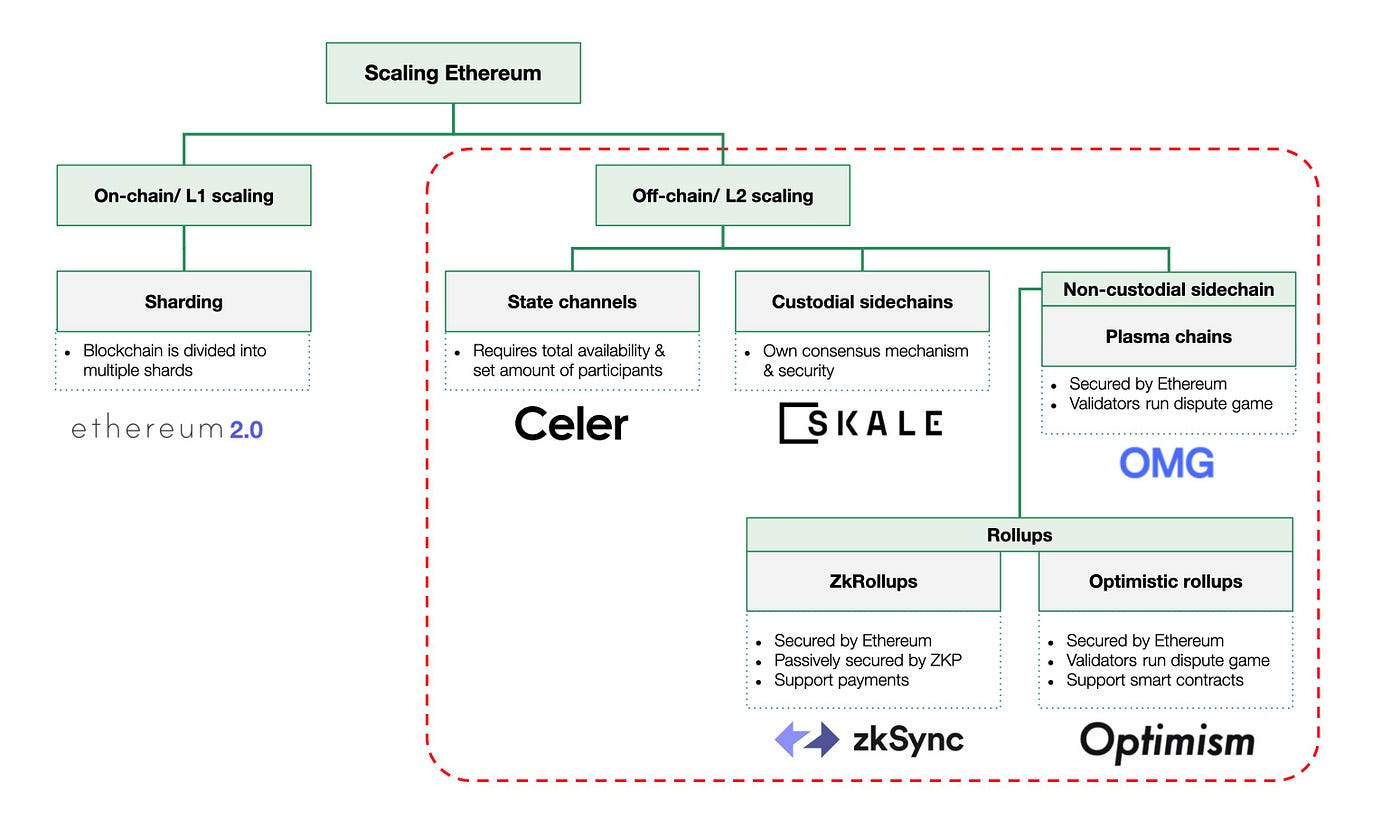
\includegraphics[width=0.95\columnwidth]{2_scalingSolutions.jpg}
  \caption[Scaling Solutions]{The current main scaling solutions for L1 and L2 \footnotemark}  
  \label{fig:2_scalingSolutions}
\end{figure} 
\footnotetext{\url{https://medium.com/token-terminal/a-primer-on-ethereum-l2-scaling-techniques-17ac437891b1}}

\subsection{Zk-Rollups}
\label{sec:2_zkRollups}
Zk-Rollups are a Layer 2 solution that uses zero-knowledge proofs to move and execute the computation off-chain. When the computation is done the results and a proof of verifiable correct computation are sent back to the blockchain smart contract. The proof is then verified by the smart contract and the results are stored on the blockchain only if the proof is verified \cite{tyagi_study_2021}.

Figure \ref{fig:2_zkRollup_schema} shows the general schema of a Zk-Rollup. The user sends a transaction to the off-chain node. The node executes the transaction batch and sends the results and a proof to the smart contract. The smart contract verifies the proof and stores the new account balance list.

\begin{figure}[ht]
  \centering
  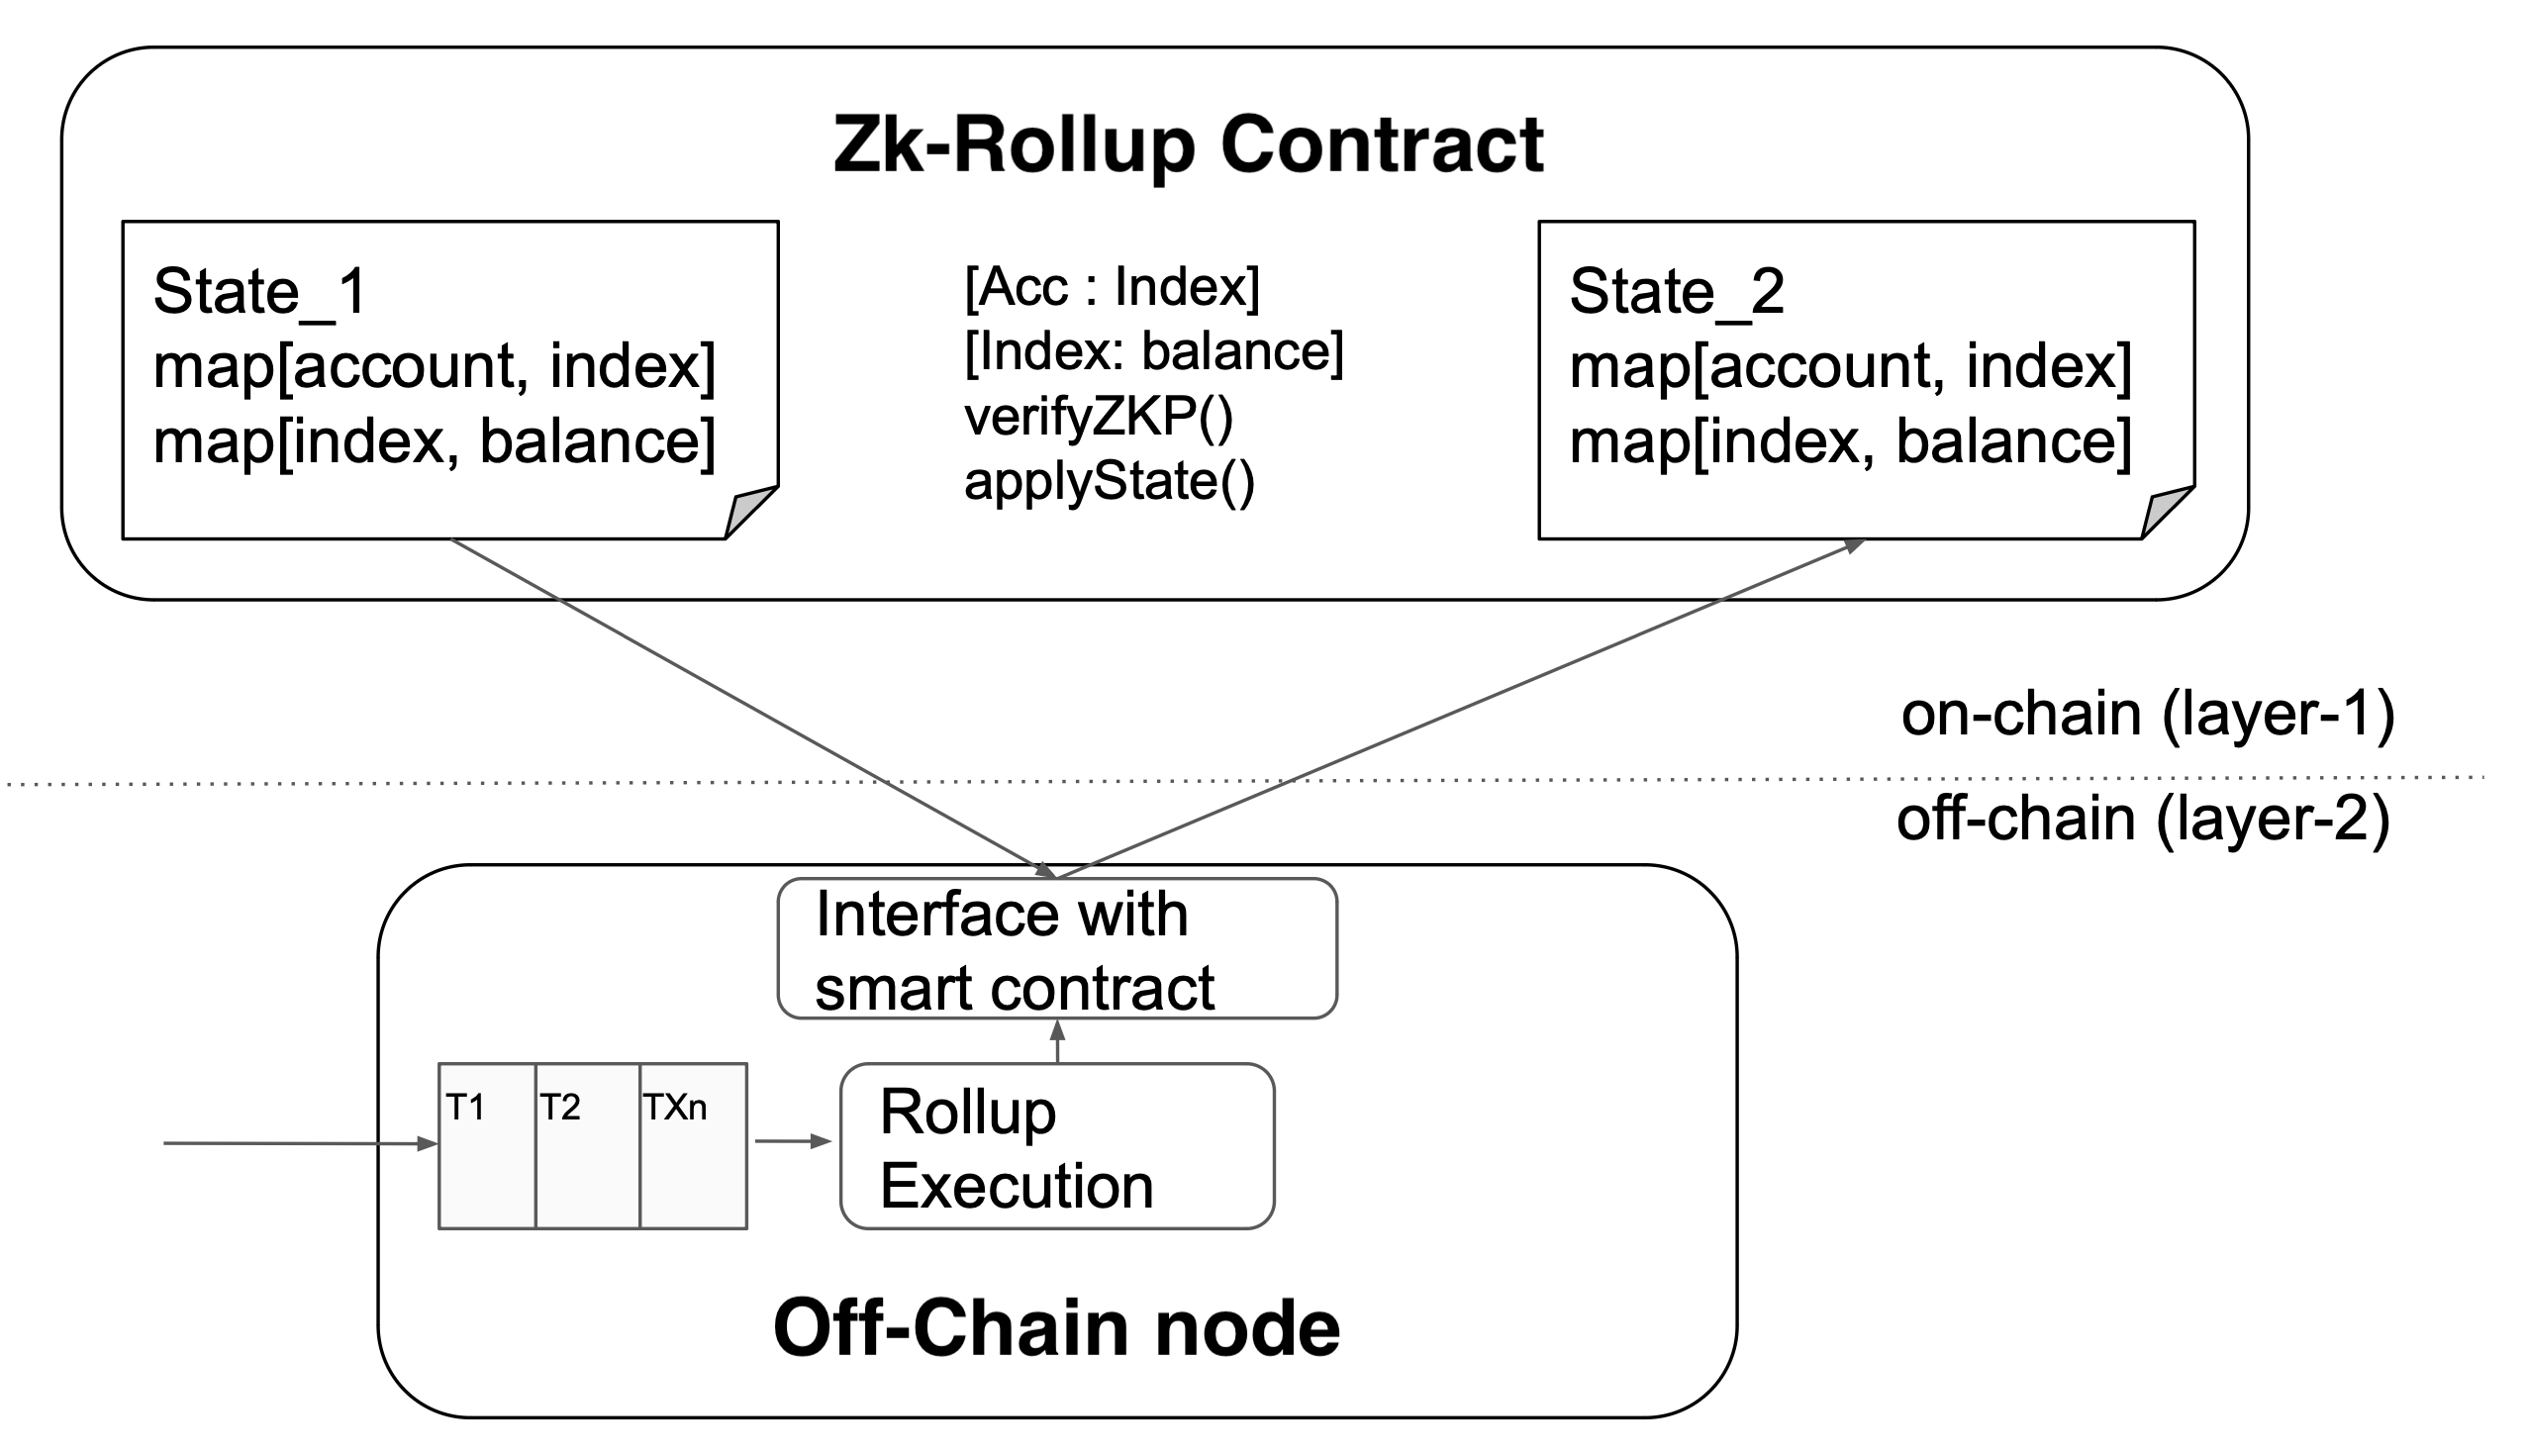
\includegraphics[width=0.95\columnwidth]{2_zkRollup_architecture.png}
  \caption[Zk-Rollup schema]{The Zk-Rollup general schema \cite{noauthor_material_nodate}}  
  \label{fig:2_zkRollup_schema}
\end{figure}

\section{ADSP Project: \textit{Scale Tezos Blockchain with Zk-Rollups}}
During the Winter Semester 2022/2023 at the University of Berlin, I worked on a project with the ADSP (Advanced Distributed Systems Prototype) group. The goal of this project was to scale the Tezos blockchain with Zk-Rollups using the ZoKrates toolbox. ZoKrates is a toolbox for zkSNARKs on Ethereum: it allows developers to write zero-knowledge proofs in a high-level programming language and generate trusted setup parameters and zero-knowledge proofs.\footnote{\url{https://github.com/ZoKrates/ZoKrates}}

\begin{figure}[ht]
  \centering
  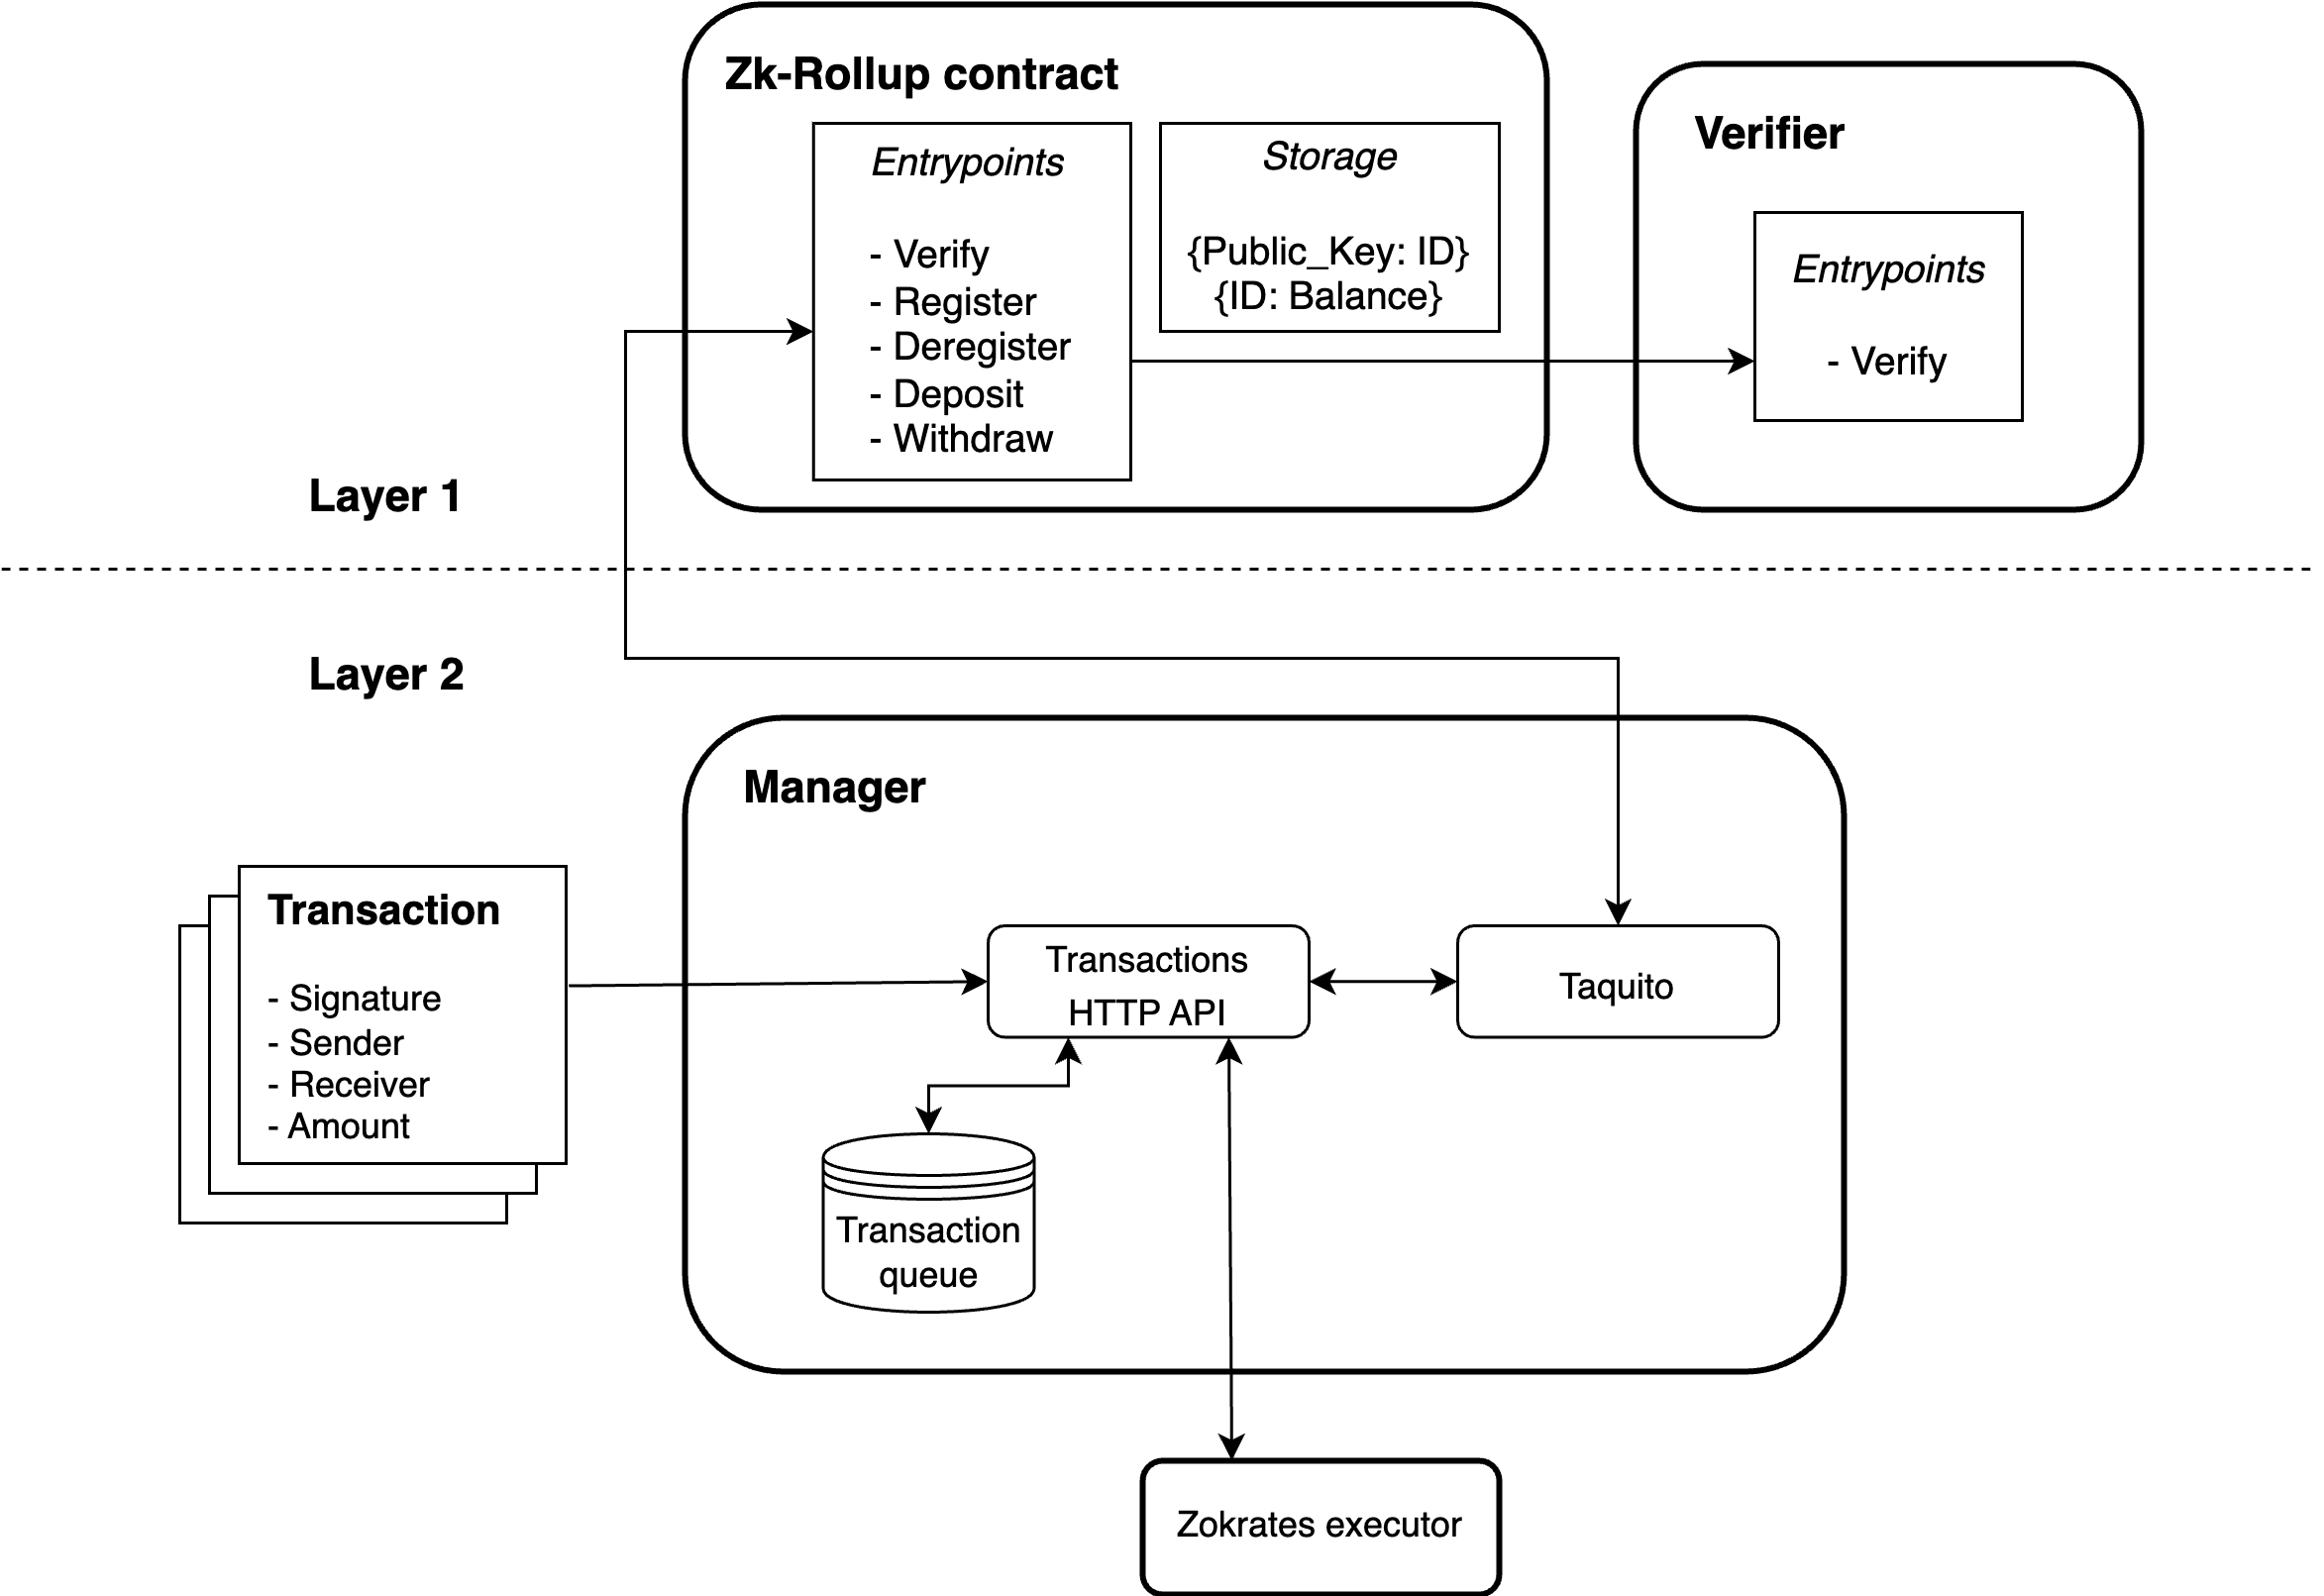
\includegraphics[width=0.95\columnwidth]{2_general_rollup_architecture.png}
  \caption[Zk-Rollup architecture]{General Zk-Rollup architecture}  
  \label{fig:2_general_rollup_architecture}
\end{figure}

The group managed to implement only a part of the prefixed objectives leaving it as a proof of concept. The system architecture is split in layer 1 and layer 2 components: the layer 1 includes the two smart contract responsible to keep the state of the system and verify the proofs; the layer 2 includes the node that executes the transactions inside the ZoKrates program that generates the proofs to be sent to the smart contract. Figure \ref{fig:2_general_rollup_architecture} shows the complete system.

The flow of a complete rollup execution is the following:
\begin{enumerate}
    \item The user sends a transaction to the off-chain node running a NodeJS server, the manager.
    \item The manager stores the transaction in a transaction queue.
    \item After 3 transactions the node executes the transaction batch spawning the process of the ZoKrates executor.
    \item The ZoKrates executor executes the ZoKrates program with the transaction batch as input.
    \item The ZoKrates executor generates the proof and the new balance list and sends them back to the NodeJS server.
    \item The NodeJS server converts the outputs of ZoKrates to a suitable format for Tezos.
    \item The converted outputs are sent to the Tezos Zk-Rollup smart contract.
    \item The smart contract forwards the payload to the verifier smart contract.
    \item The verifier smart contract verifies the proof and returns the result to the smart contract.
    \item If the proof is verified the new balance list is stored on the blockchain in the storage of the Zk-Rollup contract.
\end{enumerate}

\subsection{Developed parts}
The team developed correctly the Zk-Rollup \textit{Verify} entrypoint for the \textit{Zk-Rollup contract} and the \textit{NodeJS Manager}. The storage is also correctly implemented.

The ZoKrates program is half developed. What has been implemented is:
\begin{itemize}
    \item Check for an account to belong to the rollup system.
    \item Check for the balance of the sender account to be enough.
    \item Execution of the transaction.
    \item Output of the new balance root, the new balance list and the proof.
\end{itemize}
There wasn't the possibility to execute the signature check inside the ZoKrates program. This is due to the elliptic curves that Tezos uses, that are different from the ones of Ethereum (that is fully supported by ZoKrates).

\subsection{Missing parts \label{subsec:missingParts}}
Many are the missing parts of the project. The most important ones are:
\begin{itemize}
  \item Register entrypoint.
  \item Deregister entrypoint.
  \item Deposit entrypoint.
  \item Withdraw entrypoint.
  \item Signature check inside the ZoKrates program.
  \item Double spending problem.
  \item Optimization of the system.
\end{itemize}
A benchmarking study with single and multiple nodes is also missing, along with a security analysis and a cost comparison analysis with other scaling solutions.

\section{Other Zk-Rollup implementations}
There are many other Zk-Rollup implementations, most of them are for the Ethereum blockchain. The one developed in \cite{dinh_implementation_2023} has a similar approach to the ADSP project implementation, but they didn't consider the scaling of the system and the transfer of multiple types of tokens. The Polygon solution, Polygon Zero\footnote{\url{https://polygon.technology/blog/introducing-plonky2}}, allows transactions to be executed on L2, and the proof of the correct execution is done in parallel by all the nodes participating to the network: they combine both STARK and SNARK to achieve this, differently than the approach presented for this thesis.

\section{Reviews of Zk-Rollup}
Some studies have been done about the feasibility and the performance of the Zk-Rollup system. \cite{capko_state_2022} Gives an overview of the different zero-knowledge proofs that are mostly used. The ZoKrates Toolbox, the one used by the ADSP project, uses SNARK which is a zero-knowledge proof system having the disadvantage of requiring an initial trusted setup phase that can be a problem for some applications, compared for instance to Transparent zk-SNARK \cite{zhou_overview_2022}. \cite{neiheiser_practical_2023} Explains how the L2 solutions can face a big bottleneck in the scalability of the system due to the slow L1. All the L2 solutions analyzed in this study are limited by the low throughput of the L1 that doesn't allow them to reach the theoretical throughput of the L2. This may be a problem for some applications, in fact the idea of L3 has been proposed in \cite{starkware_fractal_2021}, to overcome this problem.

\section{Other L2 solutions}
There are some other main solutions to scale blockchains on a Layer 2. Here we will see briefly some of them.

Plasma: Plasma is a framework for creating child chains or sidechains that can handle a large number of transactions off-chain, while still being anchored to the main blockchain for security. Plasma chains can process transactions more quickly and at lower fees, but require a period of time during which watchers must be able to call for a dispute resolution over a possible fraudulent transaction \cite{thibault_blockchain_2022}. An example of network using Plasma was the OMG Network \footnote{\url{https://docs.omg.network}}.

State Channels: State channels are off-chain payment channels that allow users to transact with each other directly without needing to interact with the main blockchain. State channels enable fast, low-cost transactions and can be used for various use cases such as micropayments, gaming, and more \cite{negka_blockchain_2021}. Perun is an example of a state channel implementation \footnote{\url{https://perun.network/wp-content/uploads/Perun2.0.pdf}}.


Optimistic Rollups: Optimistic Rollups are a type of rollup that assumes transactions are valid by default and only requires verification in case of a dispute. This allows for faster and more efficient transactions, with the added security of the main blockchain as the ultimate arbiter in case of disputes \cite{thibault_blockchain_2022}.
